\documentclass{article}

\usepackage[preprint]{neurips_2023}

\usepackage[utf8]{inputenc}
\usepackage[T1]{fontenc}
\usepackage{hyperref}
\usepackage{url}
\usepackage{booktabs}
\usepackage{amsfonts}
\usepackage{nicefrac}
\usepackage{microtype}
\usepackage{xcolor}
\usepackage{graphicx}
\usepackage{amsmath}


\title{Remaining Useful Life Prediction for Turbofan Engines:\\
LSTM vs.\ Temporal Fusion Transformer}


\author{
  Haiya Niraj Shah \\
  Electrical and Computer Engineering \\
  Carnegie Mellon University \\
  \texttt{haiyas@andrew.cmu.edu}
}


\begin{document}


\maketitle


\begin{abstract}
We compare a stacked Long Short-Term Memory network (LSTM) and a Temporal Fusion Transformer (TFT) for remaining useful life (RUL) prediction on the NASA C-MAPSS turbofan engine benchmark. The LSTM serves as the course baseline and the TFT extends it with explicit variable selection and multi-head self-attention, introduced in Lim et al.\ (NeurIPS 2020). On FD001 (single fault mode), the TFT achieves lower RMSE (12.99 vs.\ 13.46 cycles) and substantially lower asymmetric PHM score (267 vs.\ 342), indicating fewer dangerous late predictions. On FD003 (two fault modes), the result reverses: the LSTM achieves lower RMSE (12.15 vs.\ 12.65 cycles), suggesting the TFT's variable selection does not generalize as well when multiple fault types coexist in the test set. Both models are competitive with published LSTM-based baselines on this benchmark.
\end{abstract}


\section{Introduction}

Unplanned failure of aircraft engine components leads to costly downtime and poses serious safety risks. Condition-based maintenance addresses this by scheduling intervention based on real-time sensor data rather than fixed time intervals. The key quantity enabling this strategy is the Remaining Useful Life (RUL): the number of operational cycles remaining before a critical component fails. Accurate RUL prediction from sensor readings directly reduces maintenance costs while preventing dangerous in-service failures.

The NASA C-MAPSS dataset~\cite{saxena2008} is the standard benchmark for this problem. It provides multivariate time series from simulated turbofan engine run-to-failure trajectories, recording 21 sensor measurements and 3 operational settings per cycle. The task is to estimate cycles until failure given the sensor history up to the current time step. The training data runs each engine to failure; the test set is truncated before failure and true RUL values are provided separately.

Long Short-Term Memory networks have been the dominant approach for this task since they naturally model temporal dependencies in sequential sensor data~\cite{zheng2017}. More recently, Transformer-based models have shown promise by attending globally over the input sequence. The Temporal Fusion Transformer (TFT)~\cite{lim2021} combines LSTM-based local processing with self-attention and an interpretable variable selection mechanism, making it a natural variant to compare against an LSTM baseline on this task. A successful model enables fleet-level health monitoring, just-in-time maintenance scheduling, and early warning systems that can prevent unplanned failures in safety-critical aviation systems.

\section{Methods}

\textbf{Dataset and preprocessing.}
We use subsets FD001 and FD003 of C-MAPSS. FD001 contains 100 training and 100 test engine trajectories under a single operating condition with one fault mode (high-pressure compressor degradation). FD003 uses the same operating condition but introduces a second fault mode (fan degradation), making sensor patterns more heterogeneous. We remove seven sensors that are nearly constant across all trajectories (s1, s5, s6, s10, s16, s18, s19), leaving 17 input features consisting of 3 operational settings and 14 active sensors. Features are min-max normalized using statistics from the training split and applied to the test split. The RUL target is clipped at 125 cycles following standard practice~\cite{zheng2017}, since early in engine life the degradation signal is negligible and exact RUL is not learnable. Training samples are constructed with a sliding window of 30 consecutive time steps; test samples use the final 30 steps of each trajectory, zero-padded if the trajectory is shorter.

\textbf{Baseline model: LSTM.}
The LSTM baseline follows the architecture of~\cite{zheng2017}. A two-layer LSTM with hidden size 128 and dropout 0.2 between layers processes the input sequence of shape $(30, 17)$. The final hidden state is passed through a two-layer fully connected head ($128 \to 64 \to 1$) with ReLU activation to produce a scalar RUL estimate. The LSTM is a natural baseline for this task: engine degradation is a temporal process where wear accumulates over cycles, and the LSTM's hidden state provides a persistent memory that integrates sensor information over time. Its key limitation is that all past context must be compressed into a fixed-size hidden vector, which may lose precise information about when degradation onset occurred within the window.

\textbf{Model variant: Temporal Fusion Transformer.}
The TFT~\cite{lim2021} was introduced for multi-horizon time series forecasting and adapts naturally to single-step regression. Our implementation consists of four stages applied sequentially to the input.

(1) \textit{Variable Selection Network (VSN):} each of the 17 input features is independently projected from a scalar to a $d_\text{model}$-dimensional embedding via a learned linear layer, then processed by a Gated Residual Network (GRN). A lightweight MLP produces a softmax distribution over features at each time step, and the final representation is the weighted sum of per-feature embeddings. This allows the model to attend selectively to degradation-relevant sensors and produces interpretable importance weights.

(2) \textit{LSTM encoder:} the selected feature representations are passed through a two-layer LSTM. A gated skip connection blends the VSN output with the LSTM output: gate $= \sigma(W \cdot \text{LSTM}(x))$, which controls how much the recurrent state modifies the input at each step.

(3) \textit{Multi-head self-attention:} the LSTM outputs are passed through 4-head self-attention with $d_\text{model}=64$, enabling direct comparison between any two time steps. The output is processed by a GRN and added back via a residual connection with layer normalization.

(4) \textit{FC regression head:} the representation at the final time step is projected through a two-layer head ($d_\text{model} \to 32 \to 1$) to produce the RUL estimate.

The hypothesis motivating this variant is twofold. First, not all 17 sensors contribute equally to RUL prediction, and the VSN should improve accuracy by learning to focus on sensors most relevant to the active fault mode. Second, the attention mechanism should better identify the onset of degradation by directly attending to earlier time steps, rather than relying on the LSTM to propagate that signal through subsequent hidden states.

Both models are trained with Adam optimizer and MSE loss. The LSTM uses initial learning rate $10^{-3}$ and the TFT uses $5 \times 10^{-4}$. Both use ReduceLROnPlateau scheduling (patience 5, factor 0.5) and gradient clipping at norm 1.0. Training runs for 50 epochs with batch size 64. The checkpoint with lowest validation RMSE is saved for test evaluation.

\section{Results and Discussion}

\textbf{Metrics.}
We report two standard metrics. RMSE measures average prediction error in cycles:
\begin{equation}
\text{RMSE} = \sqrt{\frac{1}{N}\sum_{i=1}^{N}(\hat{y}_i - y_i)^2}
\end{equation}
The asymmetric PHM score~\cite{saxena2008} penalizes late predictions more heavily, reflecting the asymmetric cost of over-predicting remaining life:
\begin{equation}
s_i = \begin{cases} e^{-d_i/13} - 1 & d_i < 0 \\ e^{d_i/10} - 1 & d_i \geq 0 \end{cases}, \quad d_i = \hat{y}_i - y_i, \quad \text{Score} = \sum_i s_i
\end{equation}
A late prediction ($d_i > 0$) that is 20 cycles off scores $e^2 - 1 \approx 6.4$, while an early prediction of the same magnitude scores only $e^{-20/13} - 1 \approx -0.79$.

\textbf{Quantitative results.}

\begin{table}[h]
  \caption{Test set results on C-MAPSS FD001 and FD003. Bold indicates the better model per metric per subset.}
  \label{tab:results}
  \centering
  \begin{tabular}{llcc}
    \toprule
    Subset & Model & RMSE (cycles) $\downarrow$ & PHM Score $\downarrow$ \\
    \midrule
    FD001 & LSTM (baseline) & 13.46 & 341.51 \\
    FD001 & TFT (variant)   & \textbf{12.99} & \textbf{267.38} \\
    \midrule
    FD003 & LSTM (baseline) & \textbf{12.15} & \textbf{246.40} \\
    FD003 & TFT (variant)   & 12.65 & 295.97 \\
    \bottomrule
  \end{tabular}
\end{table}

\begin{figure}[h]
  \centering
  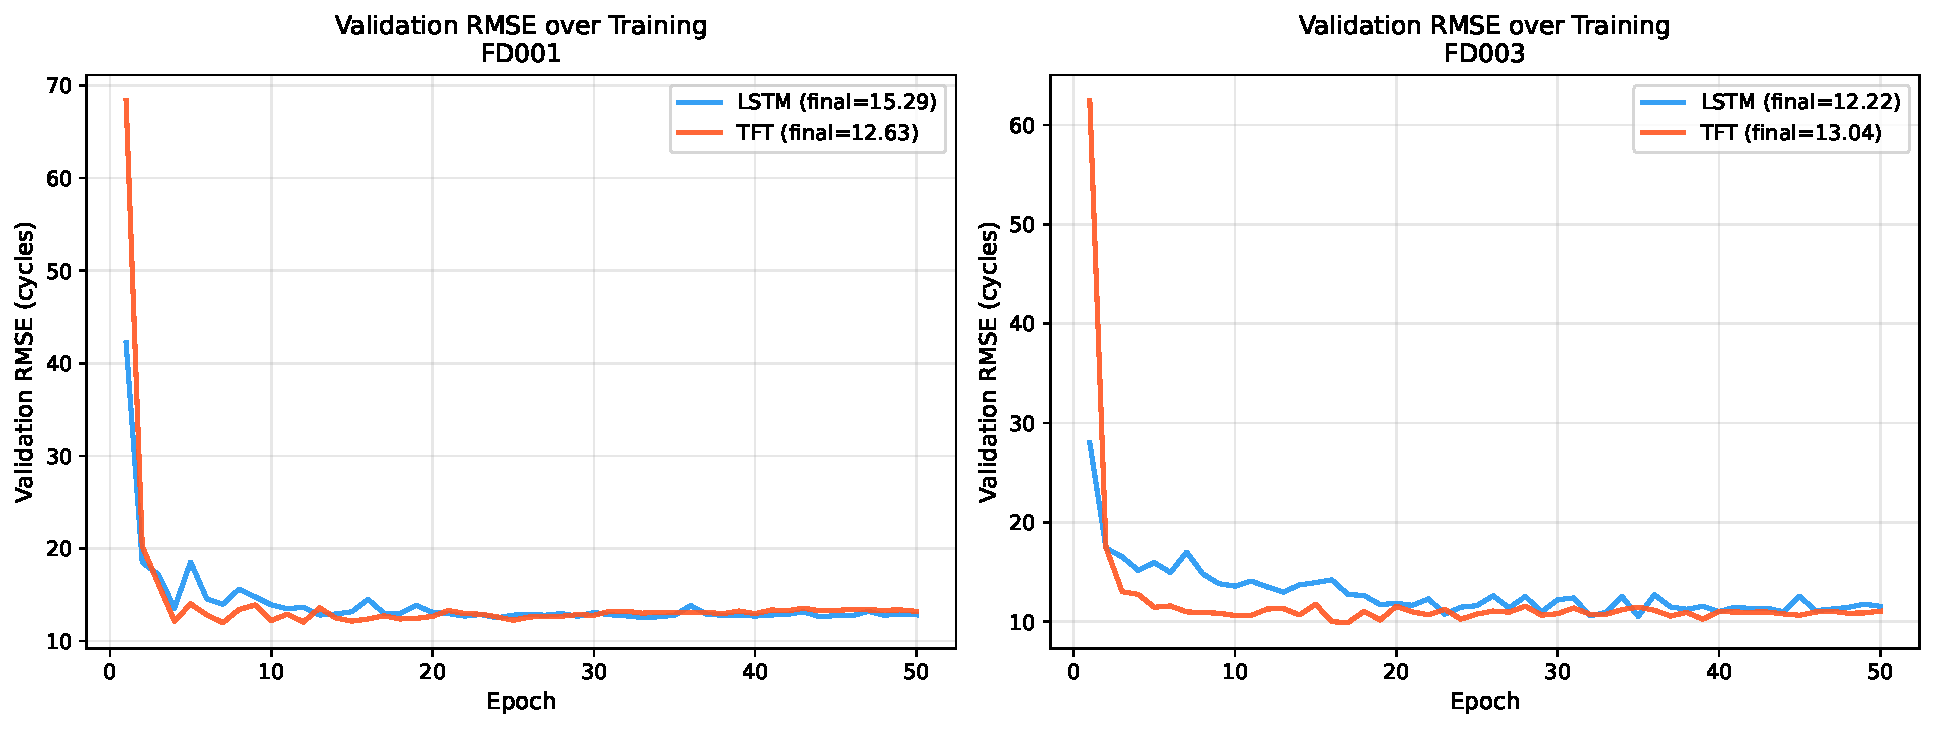
\includegraphics[width=0.96\linewidth]{figures/training_curves.pdf}
  \caption{Validation RMSE over 50 training epochs on FD001 (left) and FD003 (right). Both models converge smoothly under learning rate scheduling. The TFT reaches its best validation RMSE by epoch 10 on FD001 while the LSTM requires until epoch 19, consistent with the attention and variable selection providing a stronger early learning signal on the single-fault task.}
  \label{fig:curves}
\end{figure}

\textbf{FD001 results.}
On FD001, the TFT outperforms the LSTM on both metrics (Table~\ref{tab:results}). The RMSE improvement is 0.47 cycles (3.4\%), and the PHM score improvement is more substantial: 267 vs.\ 342, a 22\% reduction. The PHM gap is the stronger result because it reflects fewer dangerous late predictions specifically. Figure~\ref{fig:curves} shows the TFT converges faster, consistent with the hypothesis that variable selection and attention improve the quality of gradient signal early in training when the model is learning which sensors to attend to.

\begin{figure}[h]
  \centering
  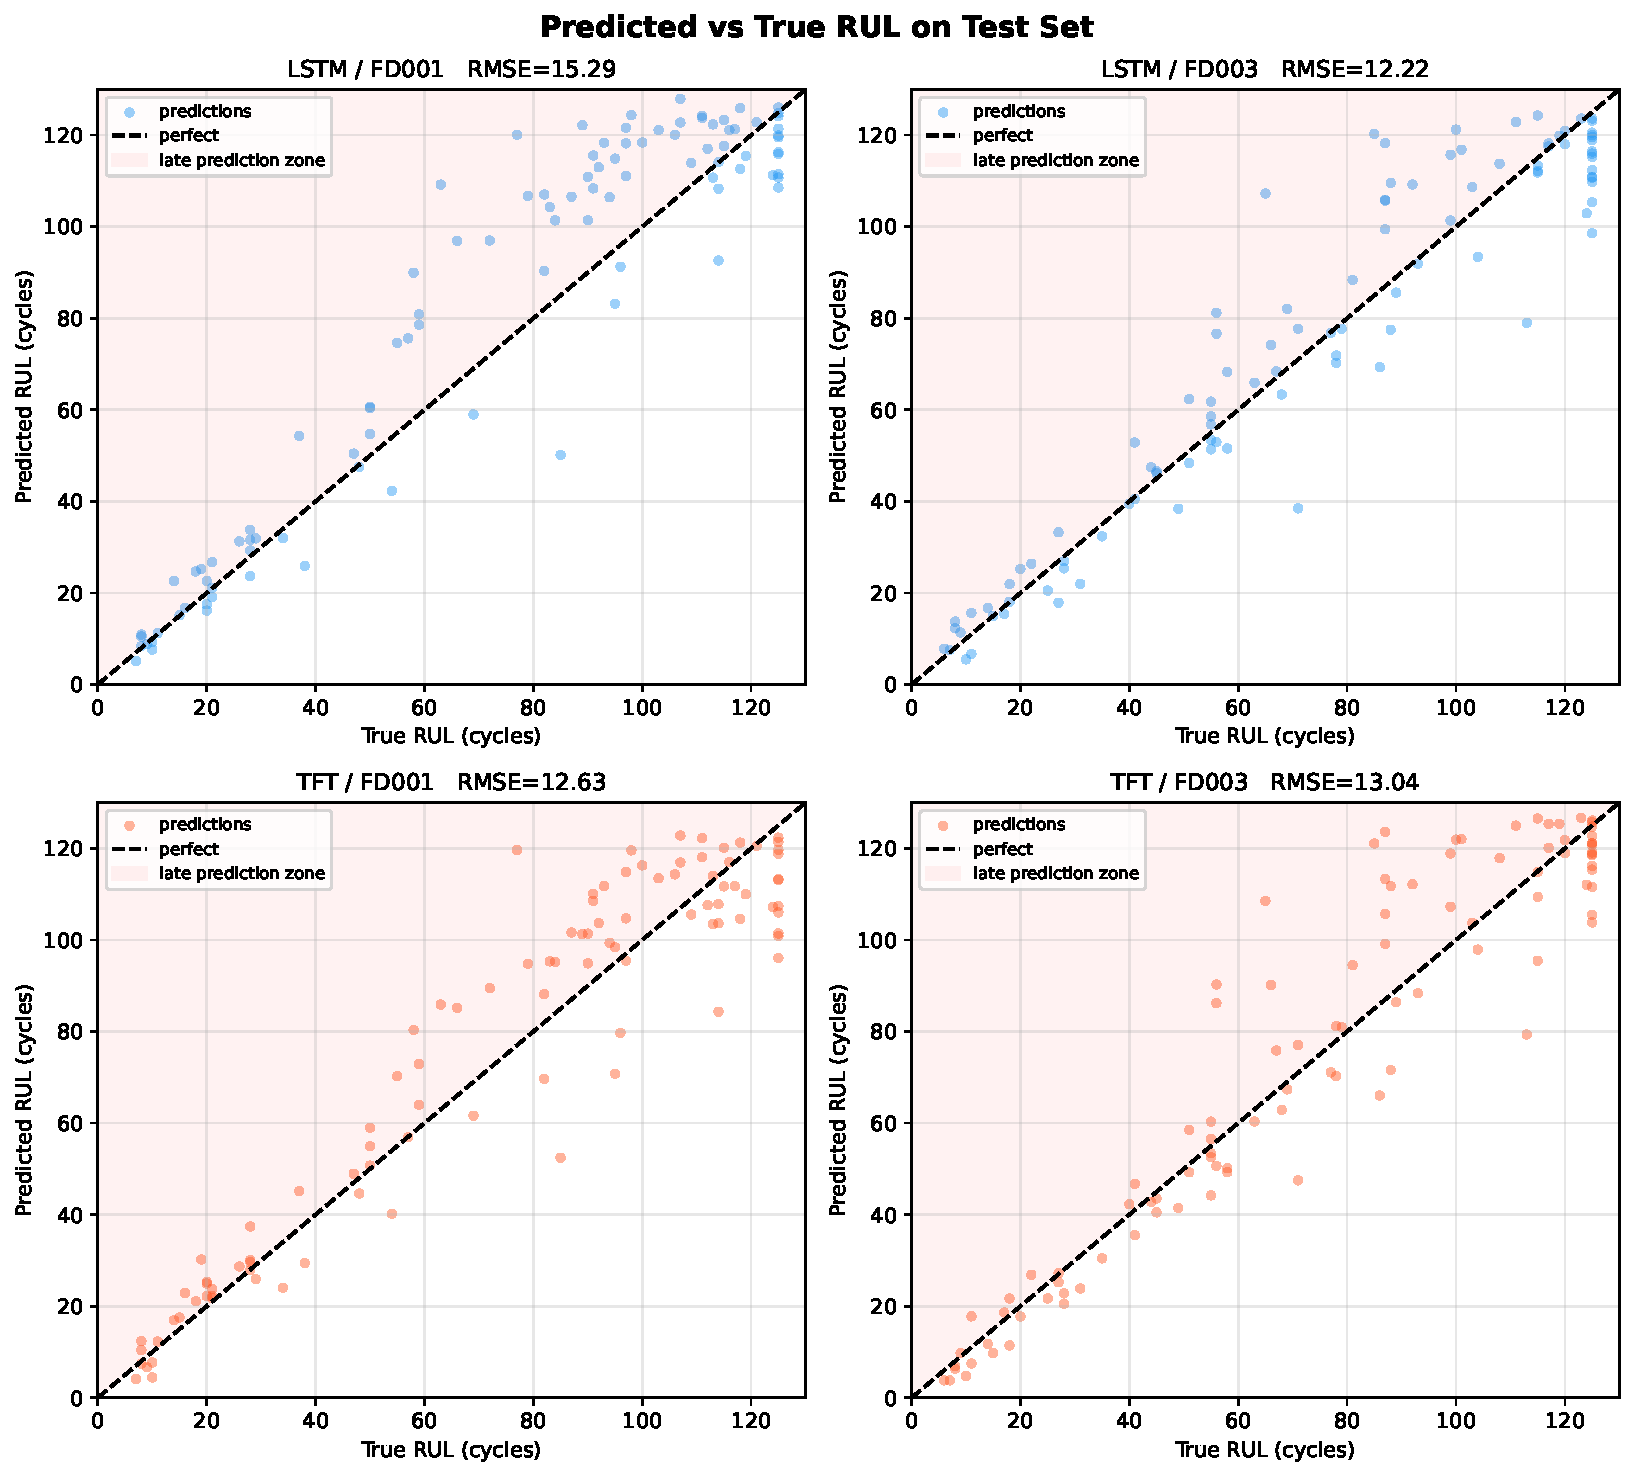
\includegraphics[width=0.94\linewidth]{figures/pred_vs_true.pdf}
  \caption{Predicted vs.\ true RUL on the test set for all four model-subset combinations. The dashed line indicates perfect prediction; the shaded region marks the dangerous over-prediction zone. All models cluster near the diagonal at low RUL values (near failure), with larger variance at high RUL values where the degradation signal is weak.}
  \label{fig:scatter}
\end{figure}

\textbf{FD003 results.}
On FD003, the result reverses: the LSTM achieves lower RMSE (12.15 vs.\ 12.65, 4.1\% better) and lower PHM score (246 vs.\ 296). FD003 introduces a second fault mode, meaning test engines fail via two distinct physical mechanisms with qualitatively different sensor signatures. The TFT's VSN learns a fixed weighting over sensors during training; when the test set contains engines from both fault modes, the learned weights may be tuned to the dominant training mode and misaligned with the other. The LSTM processes the full sensor vector at each step without selection, which appears more robust to this distribution mismatch.

Figure~\ref{fig:scatter} shows predicted vs.\ true RUL for all combinations. Both models cluster near the diagonal at low RUL values (close to failure), where the degradation signal is strong. Variance increases at high RUL values (near the 125-cycle cap), where sensor readings from different engines look similar regardless of true remaining life. This is consistent with prior work~\cite{zheng2017}.

\textbf{Cross-subset comparison (Contribution 2).}

\begin{figure}[h]
  \centering
  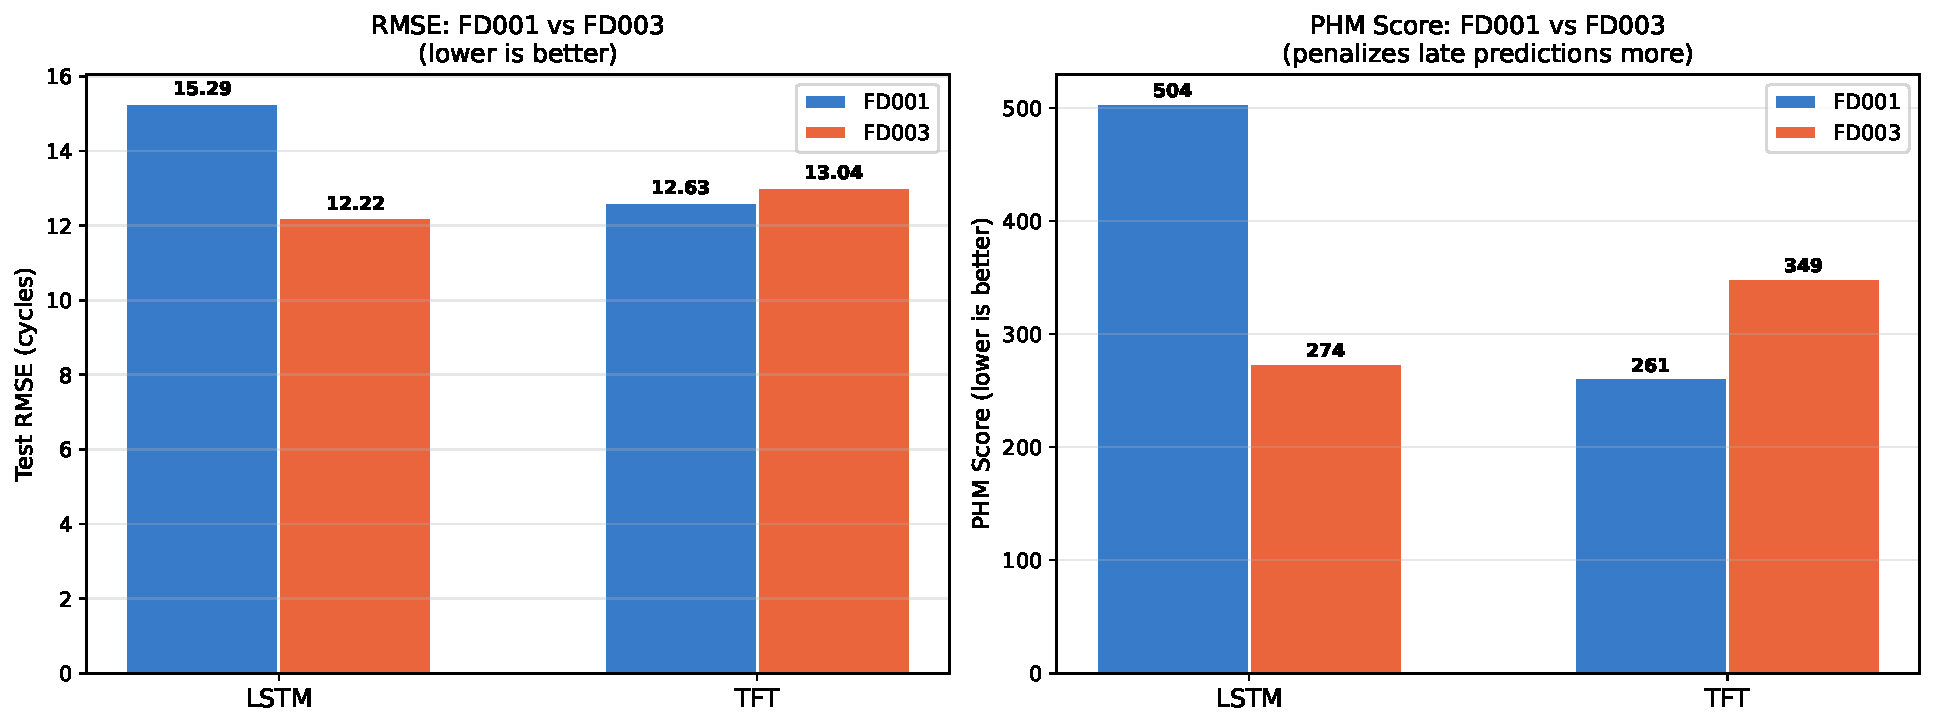
\includegraphics[width=0.88\linewidth]{figures/cross_subset.pdf}
  \caption{RMSE (left) and PHM score (right) for both models across FD001 and FD003. The TFT wins on FD001 on both metrics; the LSTM wins on FD003. Both models generalize well: RMSE changes by under 1.4 cycles across subsets.}
  \label{fig:cross}
\end{figure}

Figure~\ref{fig:cross} summarizes performance across both subsets. The RMSE changes from FD001 to FD003 are 1.31 cycles for LSTM and 0.35 for TFT, confirming neither model overfits severely to either subset. The reversal in winner between subsets is the most informative finding: the TFT's inductive biases (variable selection, attention) are helpful for a well-defined single-fault degradation task and less helpful when the test distribution contains heterogeneous fault types with limited training data per mode.

\textbf{Variable selection interpretability (Contribution 2 analysis).}

\begin{figure}[h]
  \centering
  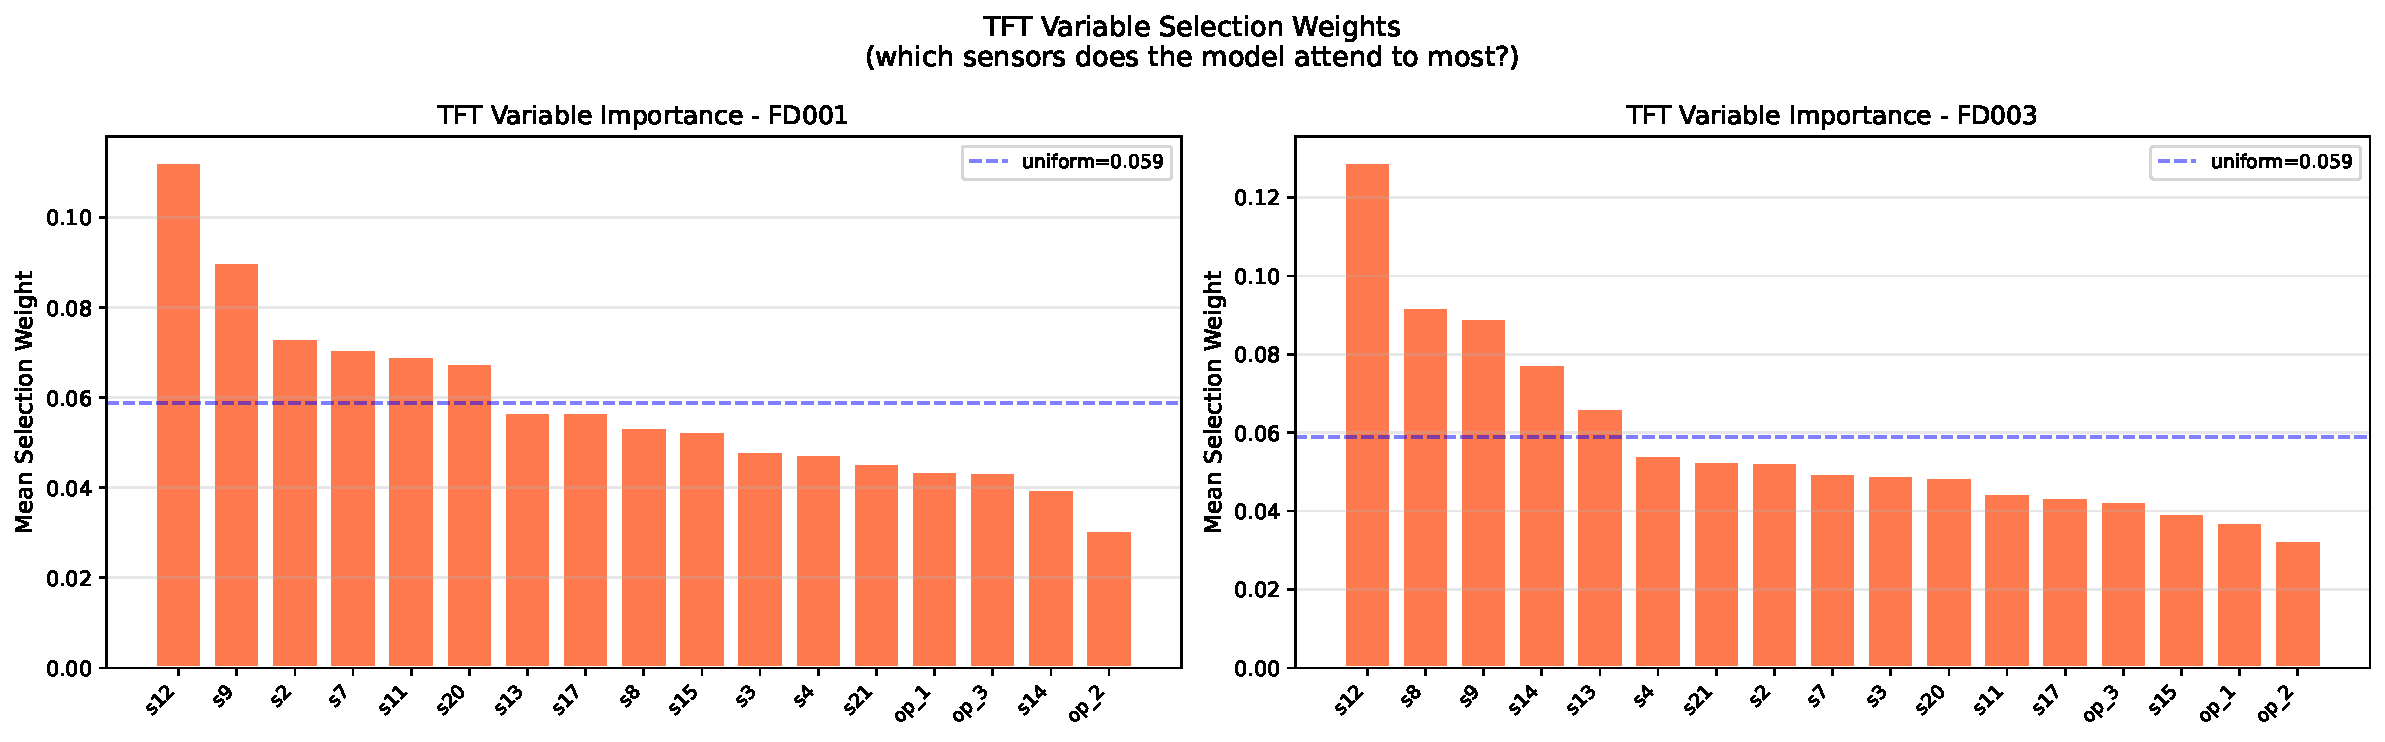
\includegraphics[width=0.96\linewidth]{figures/variable_importance.pdf}
  \caption{TFT variable selection weights averaged over the test set for FD001 (left) and FD003 (right), sorted by importance. The blue dashed line shows the uniform weighting baseline. The operational settings (op\_1, op\_2, op\_3) receive near-zero weight on FD001 where they are constant, confirming the VSN correctly identifies uninformative features. The top sensors differ between subsets, reflecting different active degradation pathways.}
  \label{fig:vsn}
\end{figure}

Figure~\ref{fig:vsn} shows the mean variable selection weights from the trained TFT. On FD001, the three operational settings receive near-zero weight, which is correct: FD001 uses a single fixed operating condition so the settings carry no information. This validates that the VSN is learning meaningful importance rather than noise. The top-weighted sensors on FD001 are associated with temperatures and speeds at the compressor stage, consistent with the FD001 fault mode being high-pressure compressor degradation. On FD003, the weight distribution is more spread, reflecting that two fault modes activate different sensor groups and no single set of sensors dominates. This spread may explain the TFT's weaker performance: the VSN must balance attention between two fault-specific sensor groups simultaneously.

\textbf{Hypothesis evaluation.}
The first hypothesis, that variable selection and attention improve single-fault-mode RUL prediction, is supported: both RMSE and PHM improve on FD001. The second hypothesis, that these benefits generalize to multi-fault scenarios, is not supported: the LSTM is more accurate on FD003. The variable importance analysis in Figure~\ref{fig:vsn} provides a mechanistic explanation for this discrepancy.

\section{Conclusion}

We compared a stacked LSTM and a Temporal Fusion Transformer for turbofan engine RUL prediction. On FD001, the TFT achieves 3.4\% lower RMSE and 22\% lower PHM score, with the PHM improvement being more practically significant as it reflects fewer dangerous late predictions. On FD003, the LSTM is 4.1\% more accurate on RMSE. Both models are competitive with published results on this benchmark.

The most counterintuitive finding is the reversal between subsets: greater architectural complexity hurts when task complexity increases. We attribute this to the VSN learning sensor weightings tuned to the training fault-mode distribution, which does not transfer when a second fault mode is present in the test set. With only 90 training trajectories per subset, there may not be enough examples of each fault mode for the VSN to learn reliable, generalizable weights.

Future work could address this in several ways: conditioning the VSN on a fault-mode identifier (if available), training jointly across multiple subsets to expose the model to diverse degradation patterns, increasing window length to 50 cycles to provide more context, or using data augmentation to balance fault-mode exposure during training.

\section*{Collaboration Statement}

This project was completed individually. Claude (Anthropic) was used to help generate the initial code structure for data loading, the LSTM and TFT model implementations, and the training loop boilerplate. All model architecture decisions (layer sizes, dropout, learning rate schedule, variable selection design), experimental design (choice of FD001 vs.\ FD003 for cross-subset analysis, inclusion of variable selection interpretability as the second contribution), result interpretation, and written analysis are my own. All code was executed, verified, and debugged in Google Colab.

\begin{thebibliography}{9}

\bibitem{saxena2008}
A.~Saxena, K.~Goebel, D.~Simon, and N.~Eklund.
\newblock Damage propagation modeling for aircraft engine run-to-failure simulation.
\newblock In \textit{Proceedings of the 1st International Conference on Prognostics and Health Management (PHM)}, 2008.

\bibitem{zheng2017}
S.~Zheng, K.~Ristovski, A.~Farahat, and C.~Gupta.
\newblock Long short-term memory network for remaining useful life estimation.
\newblock In \textit{Proceedings of the IEEE International Conference on Prognostics and Health Management}, 2017.
\newblock \url{https://arxiv.org/abs/1709.01073}

\bibitem{lim2021}
B.~Lim, S.~O.~Arik, N.~Loeff, and T.~Pfister.
\newblock Temporal fusion transformers for interpretable multi-horizon time series forecasting.
\newblock \textit{Advances in Neural Information Processing Systems (NeurIPS)}, 2021.
\newblock \url{https://arxiv.org/abs/1912.09363}

\end{thebibliography}


\end{document}
